\chapter{Work Breakdown}

\section{Project Schedule}


This section will outline the assumed tentative schedule for this Senior Design project. Gantt charts will be used to show the progress of this project over several revisions of this Project Plan and serve as a visual timeline of the projects accomplishments upon completion in May. The schedules below are subject to change as the need arises. 

\begin{figure}[!ht]
\centering
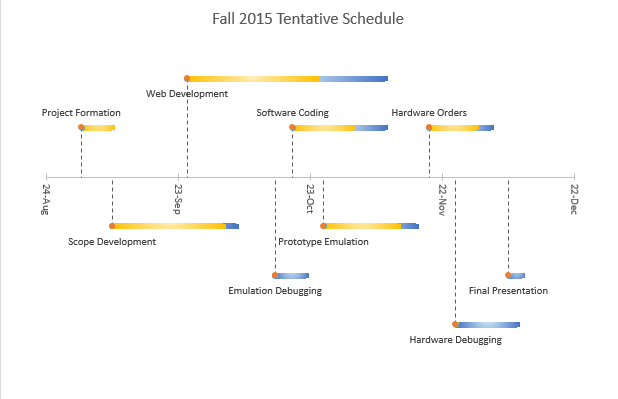
\includegraphics[scale=0.65]{./figures/fall-timeline}
\caption{Tentative Fall 2015 Project Schedule Overview}
\label{figure:fall-timeline}
\end{figure}

\begin{table}
\centering
\begin{tabular}{l  c  c  c}
Task & Start & Duration & End \\
\hline
Project Formation & 2015-09-01 & 7 & 2015-09-08 \\
Scope Development & 2015-09-08 & 28 & 2015-10-06 \\
Web Development & 2015-09-25 & 45 & 2015-11-09 \\
Emulation Debugging & 2015-10-15 & 7 & 2015-10-22 \\
Software Coding & 2015-10-16 & 21 & 2015-11-9 \\
Project Formation & 2015-10-26 & 21 & 2015-11-16 \\
Hardware Orders & 2015-11-19 & 14 & 2015-12-3 \\
Hardware Debugging & 2015-11-25 & 14 & 2015-12-9 \\
Final Presentation & 2015-12-7 & 3 & 2015-12-10 \\
\end{tabular}
\caption{Fall 2015 Detailed Project Schedule}
\label{table:risk}
\end{table}
\vspace{0.3cm}

\begin{figure}
\centering
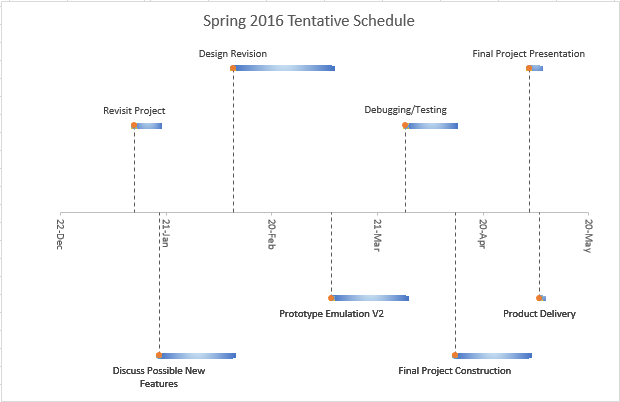
\includegraphics[scale=0.65]{./figures/spring-timeline}
\caption{Tentative Spring 2016 Project Schedule}
\label{figure:fall-timeline}
\end{figure}

\begin{table}
\centering
\begin{tabular}{l  c  c  c}
Task & Start & Duration & End \\
\hline
Revisit Project	& 2016-01-12 & 7 & 2016-01-19 \\
Discuss Possible New Features & 2016-01-19 & 21 & 2016-01-19 \\
Design Revision & 2016-02-09 & 28 & 2016-03-08 \\
Prototype Emulation V2 & 2016-03-08 & 21 & 2016-03-29 \\
Debugging/Testing & 2016-03-29 & 14 & 2016-04-12 \\
Final Project Construction & 2016-04-12 & 21 & 2016-05-03 \\
Final Project Presentation & 2016-05-03 & 3 & 2016-05-06 \\
Product Delivery & 2016-05-06 & 1 & 2016-05-07 \\
\end{tabular}
\caption{Spring 2016 Detailed Project Schedule}
\label{table:risk}
\end{table}
\vspace{0.3cm}


\section{Risks and Feasability Assessment}

This project is routinely implemented in industry with high success rates. Several software implementations of SCADA honeypots already exist in the open source community. However, our implementation will be custom because the client has a secondary goal of including an IDS on the system. Creating the honeypot software from conception will minimize the resources required from the platform. This is important because the computer needs to be a small standalone device. A standard Raspberry PI only has 512MB of RAM for example. An IDS typically uses a lot of memory and process cycles. Most risk can be mitigated with proper contingency planning, as summarized in Table \ref{table:risk}.


\vspace{0.5cm}
\begin{table}[h]
\centering
\begin{tabular}{l  c  r}
Component & Risk & Contingency Plan \\
\hline
Web Server Honeypot & Low & Utilize open source nginx\footnotemark[7] \\
SSH Server Honeypot & Low & Use open source Kippo SSH\footnotemark[8] \\
Event Alerts & Medium & Switch from REST API to SMTP \\
SCADA Honeypot & Medium & Use open source Conpot\footnotemark[9] \\
Intrusion Detection System & High &  Use IPTables Logging \\
\end{tabular}
\caption{Summary of project components and implementation risk}
\label{table:risk}
\end{table}
\vspace{0.3cm}

% handle footnotes in table
\addtocounter{footnote}{7}
\footnotetext{\url{https://www.nginx.com}}

\addtocounter{footnote}{1}
\footnotetext{\url{https://github.com/desaster/kippo}}

\addtocounter{footnote}{1}
\footnotetext{\url{http://conpot.org/}}

Installing an IDS on a small platform such as a Raspberry PI may not be feasible. If this is the case, developing a custom platform with greater processing power and more memory will be explored. If this isn't feasible, then the secondary goal will have to be canceled. However, the overall honeypot implementation carries a low risk of failure.

\section{Cost Considerations}

Alliant Energy requires service in twenty eight different locations. Each location will house a standalone minimal computer. The CanaKit Raspberry PI was chosen because it is customizable and holds more memory than standard versions. An additional network interface will also be provided from an external network adapter. \ref{table:cost}.

\vspace{0.5cm}
\begin{table}[h]
\centering
\begin{tabular}{l l l l}
Model & Unit Cost & Vendor & Total Cost \\
\hline
Raspberry PI B+ & \$69.99 Plus Tax & CanaKit & \$1960 Plus Tax\footnotemark \\
\hline
USB 3.0 Gigabit Ethernet Adapter & \$16.99 Plus Tax & Anker & \$476 Plus Tax\footnotemark\\
\end{tabular}
\caption{Summary of implementation costs}
\label{table:cost}
\end{table}
\vspace{0.5cm}

\addtocounter{footnote}{-1}
\footnotetext{\url{http://www.amazon.com/CanaKit-Raspberry-Complete-Original-Preloaded/dp/B008XVAVAW/ref=sr_1_1?s=pc&ie=UTF8&qid=1444258362&sr=1-1&keywords=raspberry+pi}}

\addtocounter{footnote}{1}
\footnotetext{\url{http://www.amazon.com/Anker-Gigabit-Ethernet-Adapter-Supporting/dp/B00NOP70EC/ref=sr_1_4?ie=UTF8&qid=1444258449&sr=8-4&keywords=usb+to+nici}}
